\documentclass[11pt,a4paper]{article}
\usepackage[T1]{fontenc}
\usepackage{lmodern,microtype,amsmath,amssymb,amsthm,booktabs,array,graphicx}
\usepackage[margin=27mm]{geometry}
\usepackage[colorlinks=true,allcolors=blue!45!black]{hyperref}
\usepackage{xcolor}
\usepackage{enumitem}
\setlength{\emergencystretch}{1.6em}
\newtheorem{theorem}{Theorem}[section]
\newtheorem{proposition}[theorem]{Proposition}
\newcommand{\dd}{\mathrm d}
\newcommand{\sech}{\operatorname{sech}}
\newcommand{\sgn}{\operatorname{sgn}}
\newcommand{\tr}{\operatorname{Tr}}
\newcommand{\ind}{\operatorname{ind}}
\newcommand{\vol}{\operatorname{vol}}
\hypersetup{pdftitle={Fermions at spherical throats of fixed-charge Nieh--Yan semi-wormholes},pdfauthor={Muacca},pdfsubject={Version 1, first release 2026-11-22}}
\title{Fermions at spherical throats of fixed-charge Nieh--Yan semi-wormholes}
\author{Muacca}
\date{Version 1\\First release: 2026-11-22}
\begin{document}
\maketitle
\begin{abstract}
A round Euclidean axion throat can carry the same classical action on both flux branches while supporting different fermion states. We consider the part of the Giddings--Strominger solution from its reflection surface to a finite boundary, with spatial section a spin spherical space form. For a massless test Weyl field the outer Atiyah--Patodi--Singer vacuum and the instantaneous Lorentzian vacuum prepared just across the first level crossing have a finite-rank covariance difference. Its trace is $s m_s$, where $s$ is the sign of the Nieh--Yan charge and $m_s$ counts the lifted Killing spinors in the contacting shell. A constant real Holst term separates the crossing from the throat; preparation between them gives zero difference. On the corresponding finite collar the relative four-component Dirac log modulus is $-2J\eta_Y(0)$ for fifteen spin lifts, with $J$ the integrated axial shift. We give the boundary domain and the order of limits for a shellwise extension to infinity. On the real three-form contour the fixed-flux bosonic Hessian has zero negative index. Integrating a continuous flux at fixed outer field adds one homogeneous even negative direction at finite radius and a Robin contribution on short collars. These are conditional state, determinant and stability comparisons for specified boundary experiments.
\end{abstract}
\begingroup\small\tableofcontents\endgroup
\section{Two boundary experiments at a common throat}
A three-form flux supports a smooth minimum of the area radius of a Euclidean three-sphere \cite{GS}. The geometry remembers the magnitude of that flux. A spinor also sees its sign through the axial component of the spin connection. Does a spinor then distinguish the two branches at the reflection surface? A boundary value at zero eigenvalue needs a domain, a Fock vacuum needs a polarization, and a determinant needs a regulator. We perform two explicit experiments with these choices fixed and compare their dependence on the same three-dimensional data.

We call the portion from the reflection surface to one outer end a \emph{semi-wormhole}, following the geometrical use in \cite{Kaul}. A quotient acts freely on every round section and leaves the radial equation unchanged. The allowed spinor modes can change substantially. Left and right order-three quotients have the same Einstein action and opposite asymmetric spin spectra. The lens space used below gives a different diagnostic: its two lowest contacting shells are absent, but its eta invariant is nonzero. This separates a measurement of occupied states at the throat from a measurement using all eigenvalues.

In the first experiment an outer Euclidean boundary prepares a terminal vacuum bra. A Lorentzian initial surface prepares an instantaneous vacuum ket. Both are transported to the same reflection surface using the chosen coframe. Only a finite-dimensional shell can distinguish the two covariances in the first crossing window. A single Weyl field counts this difference with a sign. In a Dirac field the opposite chirality cancels its vector charge and doubles its axial charge. This distinction survives even when both states have a vanishing vacuum overlap.

In the second experiment both ends carry spectral boundary conditions. The radial Dirac equation separates into pairs of mutually adjoint first-order operators. Their boundary Wronskians yield the same log ratio for every shell of a given sign. Summing that constant requires the signed degeneracies at arbitrarily large angular momentum. We continue the compact four-dimensional zeta difference before differentiating at zero. This identifies the angular factor with the ordinary Dirac eta invariant in the stated orientation. We give an independent shell-first prescription at infinity.

The background and many ingredients of the calculation have precedents. Kaul and Sengupta connected torsional instantons and the Nieh--Yan invariant \cite{Kaul}. Kim studied normalizable fermion zero modes on an Einstein--Kalb--Ramond wormhole \cite{Kim}. Neither its noncompact domain nor the absolute number of such modes specifies the collar experiment. Loges, Shiu and Sudhir found stability in the three-form representation \cite{LSS}. Marolf and Missoni retained the regular symmetric modes when solving the constraints \cite{MM}. We use their bulk scalar quadratic form and trace the endpoint terms through the change of ensemble. Other choices of field variables and boundary conditions have led to different putative negative directions \cite{HTV}. We distinguish a finite outer boundary from the limiting action at infinity.

A separate enhancement mechanism occurs in metric-affine axion gravity \cite{TY}. In their Eqs.~(12)--(14), (23)--(24), the nonminimal functions are functions of the modulus $f$ of a complex scalar. The torsion and nonmetricity coefficients multiply $\partial f$; the phase carries the PQ charge. The equations for the radius and $f$ are coupled, with $f'(0)=0$ and $f(\infty)=f_a$. Freezing $f$ removes that connection source. Here the independent metric-compatible connection couples directly to the derivative of the shift field, and its constant Holst coefficient rescales the charge kinetic term. The square root in Sec.~\ref{sec:background} follows from this one-field normalization. We make no priority claim for an increase in the Euclidean action. Our results concern specified spin lifts, outer domains and preparations.

We use the charge and lift conventions of the companion Paper~08 \cite{P08}. The signs and all angular inputs required here are specified again in Secs.~\ref{sec:background}, \ref{sec:det}. The external massless field, the identification of boundary spinors and the integration contour are physical inputs.

\section{Fixed charge and the two real sections}\label{sec:background}
Let $Y=S^3/\Gamma$ have the induced unit-radius metric, orientation and spin lift, and write $V=2\pi^2/|\Gamma|$. We take signature $(-+++)$ before continuation and choose the trace of torsion as $T^a{}_{ab}$. The real parameter $h=2\kappa^2 c_H$ multiplies the Holst term in the normalization of Paper~08. Set
\begin{equation}
 d=1+h^2,\quad P=Q_\Sigma=-p_\theta,\quad s=\sgn P,\quad c=\frac{|P|}{6V},\quad
 a=\sqrt d\,c=q_*^2,\qquad A_0=\frac{3V}{\kappa^2}.
 \label{eq:scales}
\end{equation}
We take $P\ne0$. The action consists of the Einstein--Cartan term, $\theta\,\dd(e^a\wedge T_a)$, a constant Holst density and the metric boundary term after connection elimination. The trace and axial equations for a homogeneous timelike source give axial coefficient $j=-\kappa^2\dot\theta/d=s c/q^3$ and vector coefficient $-hj$ in proper Lorentzian time. The dimensionless auxiliary connection Hessian has determinant $256d^{12}$. Its Schur complement gives the Lorentzian scalar density $-C(\nabla\theta)^2$ with $C=3\kappa^2/d$. At $h=0$ the canonical scalar is $\sqrt6\,\kappa\theta$; the contortion involves the derivative of $\kappa^2\theta$. In particular the conserved NY charge is distinguished from the integration constant for the field velocity at nonzero $h$.

The homogeneous Legendre transform fixes $p_\theta$, so that the scalar enters the Euclidean action with a positive flux potential. With lapse $N$, proper radial coordinate at $N=1$, induced outer radius $R$ and the flat reference boundary curvature, the action is
\begin{equation}
 I_P=A_0\int\left(-\frac{q\dot q^2}{N}-Nq+\frac{Na^2}{q^3}\right)\dd\tau+A_0 R^2 .
 \label{eq:action}
\end{equation}
The inner reflection surface has zero extrinsic curvature. Varying $N$ before setting it to one gives $\dot q^2=1-a^2/q^4$. Hence the outward proper acceleration at the throat is $2/q_*$. In conformal Euclidean time $\dd\tau=q\,\dd t$ this integrates to
\begin{equation}
 q_E^2=a\cosh(2t),\quad 0\le t\le T,\qquad
 T=\tfrac12\operatorname{arcosh}(R^2/a).
 \label{eq:q}
\end{equation}
The positive Lorentzian slice solves $(\dd q/\dd\tau_L)^2=a^2/q^4-1$ and $q_L^2=a\sin(2u)$ with $\dd\tau_L=q\,\dd u$. Continuation $u=\pi/4-it$ joins the two real metrics at vanishing first derivative. The section which is a maximum in Lorentzian time is the minimum of the real Euclidean radius. The positive Euclidean metric satisfies the complex-metric eigenvalue phase criterion trivially. This metric test does not specify a real contour for axion perturbations about an imaginary scalar derivative.

The closed spatial flux is constant along the regular collar. With the outward boundary orientations its two integrals cancel in the integral of the complete Nieh--Yan derivative. A single mouth therefore carries $P$ without fixing an integer four-dimensional charge on this boundary value problem. Substitution of the constraint into \eqref{eq:action} gives the regulated Hamilton principal function
\begin{equation}
 \frac{I_P(R)}{A_0}
 = R^2-2\int_{q_*}^R q\sqrt{1-a^2/q^4}\,\dd q
 = R^2-\sqrt{R^4-a^2}+a\arccos(a/R^2).
 \label{eq:principal}
\end{equation}
At infinity $I_P^\infty=\pi A_0 a/2=\pi\sqrt d\,|P|/(4\kappa^2)$. At fixed total charge this result is independent of the quotient order; at fixed density it scales with $V$. At fixed $q_*$ the infinite-end action is independent of $h$. At finite, fixed absolute $R$ one must use \eqref{eq:principal}. Changing $R$ together with the throat changes the boundary metric.

\begin{figure}[htbp]
\centering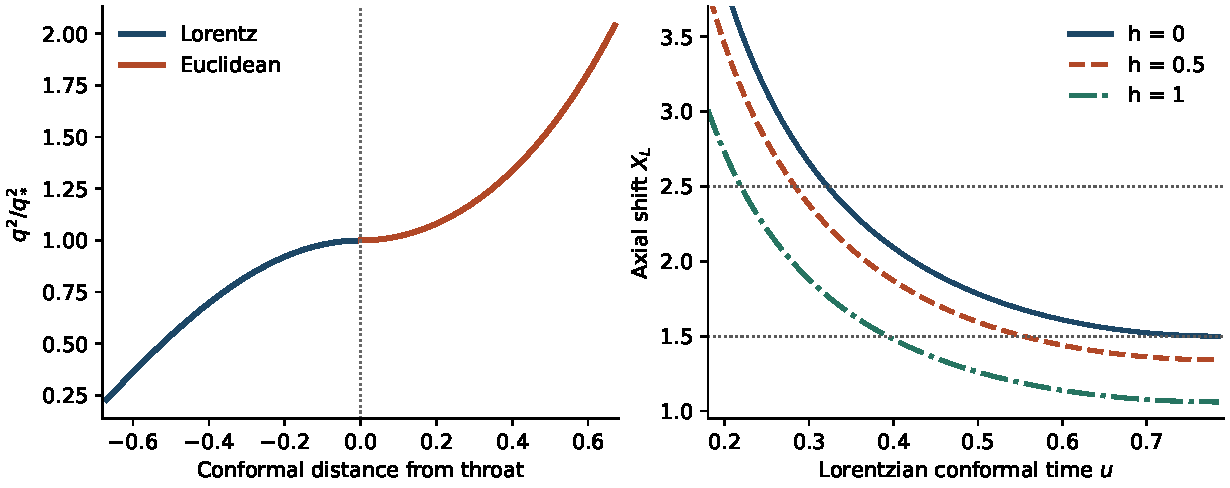
\includegraphics[width=.97\linewidth]{figures/throat.pdf}
\caption{Left: area radius squared in units of $a$ as a function of conformal distance from the reflection surface, with applications to a Lorentzian expansion and an outward Euclidean collar. Right: Lorentzian axial shift for $h=0,1/2,1$. The dashed horizontal lines are the first two absolute shell energies. The interval between the first crossing and the reflection surface is empty at $h=0$.}
\label{fig:throat}
\end{figure}

\section{Morse indices at a finite outer boundary}\label{sec:morse}
The bosonic index counts negative directions of the real gauge-invariant quadratic form, with the induced outer metric fixed. We specify the integration variable, parity at the reflection surface and outer ensemble before forming this Hessian. A real three-form $H$ has Euclidean norm term $\|H\|^2/(4C)$ and Fourier term $i\int\dd\theta\wedge H$. Completing the square in $H$ gives $+C\|\dd\theta\|^2$ for the scalar. Integrating $\theta$ first imposes $\dd H=0$. On a collar with $P\ne0$ write $H=P\omega_Y+\dd b$ with $\int_Y\omega_Y=1$. A single-valued two-form potential accounts only for the exact part. We hold $H$ fixed in ensemble E1 and remove $i\int_{\partial M}\theta H$ there. In E2 the conjugate field is fixed, and we integrate the harmonic flux over $\mathbb R$ with its Fourier kernel. A quantized flux summed over distinct bundles has different tangent data.

\begin{proposition}\label{prop:hom}
On the real three-form contour the homogeneous index for E1 is zero. For E2 at each finite $R>q_*$ there is one negative even direction and no negative odd direction. The Hessian of the infinite-boundary action has zero negative index.
\end{proposition}
\begin{proof}
The equation $\dd H=0$ constrains $P$ to one constant. At fixed $P$ the pair consisting of the scale factor and its momentum is removed by the lapse constraint and time reparametrization. In proper time the residual radial perturbation is $\delta q=\dot q\,\xi,\ \delta N=\dot\xi$. Linearizing the constraint \emph{at} the throat gives $\delta q(0)=0$ at fixed $P$, or $2q_*\delta q(0)=\delta a$ for varying flux. The odd displacement of the reflection surface is an interior coordinate translation of the smooth double. Thus no physical homogeneous radial oscillator remains at fixed flux.

For E2 first solve the metric and lapse problem at fixed $P$. The Fourier source in $\int\dd P\,e^{-iP\Delta\theta/\hbar}e^{-I_P/\hbar}$ has zero second derivative. The endpoint source must be analytically continued to the value compatible with the desired nonzero real saddle. Differentiating \eqref{eq:principal} at fixed $R$ on one sign branch gives
\begin{equation}
 I_{P,aa}= -\frac{A_0}{\sqrt{R^4-a^2}},\qquad
 \frac{\dd^2 I_P}{\dd P^2}=-\frac{A_0d}{36V^2\sqrt{R^4-a^2}} .
 \label{eq:fluxhess}
\end{equation}
The constant $\delta P$ is even. Its negative coefficient tends to zero as $R^{-2}$. The limiting action is linear in $|P|$ and the matched Fourier source leaves a flat direction on the chosen sign branch. The finite-radius index remains one for every finite radius.
\end{proof}

\paragraph{Nonconstant harmonics.}
Let $n$ denote scalar harmonic degree on the round cover, $k=n(n+2)$ and $j=k-3$. For $n\ge2$, normalize the flux variable $Q$ of \cite{MM} by $Q^2=6a^2$. Write $H_q=q'/q$, $D=3Q^2+2jq^4$. The regular gauge-invariant scalar amplitude $\mathcal R$ and its conjugate momentum have the first-order action with coefficients
\begin{equation}
 A_n=-\frac{kD}{4q^2j},\qquad
 B_n=\frac{q^2j(2jq^4-Q^2)}{D^2},\qquad p=\frac{q^2j}{kD}.
 \label{eq:weights}
\end{equation}
The imaginary momentum Gaussian leaves the real configuration form $\int(p\mathcal R'^2+B_n\mathcal R^2)\dd t$. The variable is regular at the throat since $D>0$. The factor $2jq^4-Q^2$ is at least $4a^2$. In E1 the outer boundary value vanishes, so this form is positive. In E2 the residual boundary term is $-b_T\mathcal R(T)^2$ where
\begin{equation}
 b_T=\frac{Q^2}{2 H_q(T) q(T)^2D(T)} > 0 .
 \label{eq:robin}
\end{equation}
The natural boundary condition is $p\mathcal R'(T)=b_T\mathcal R(T)$. At the throat, even fields have natural Neumann data and odd fields have Dirichlet data. Appendix~\ref{app:robin} derives the boundary form and its one-dimensional sign test. The degeneracy of $j=0$ at $n=1$ expresses a scalar gauge mode. The two metric scalar tensors there are dependent. The remaining constraints remove the boundary term with either ensemble. Transverse vectors have no vorticity source, and the shift removes the non-Killing components. Tensor harmonics have form proportional to $\int q^2(v'^2+n(n+2)v^2)\dd t$; quotient projection only reduces their multiplicity.

\begin{table}[htbp]\centering
\begin{tabular}{lrrrr}
\toprule
$Y$ & $d_2,d_3,d_4$ & E2 even at $1.1$ & E2 odd at $1.1$ & E2 at $\ge1.5$\\
\midrule
$S^3$ & $9,16,25$ & 51 & 25 & $1,0$\\
$\mathbb{RP}^3$ & $9,0,25$ & 35 & 9 & $1,0$\\
left $C_3$ & $3,8,5$ & 17 & 11 & $1,0$\\
$L(5,2)$ & $1,4,5$ & 11 & 5 & $1,0$\\
$L(7,2)$ & $1,2,3$ & 7 & 3 & $1,0$\\
left $2I$ & $0,0,0$ & 1 & 0 & $1,0$\\
\bottomrule
\end{tabular}
\caption{Total real bosonic indices at the indicated finite $R/q_*$. The last column gives even, odd. At $1.1$ the inhomogeneous even contribution is $d_2+d_3+d_4$, the odd contribution $d_2+d_3$. All E1 indices vanish. The strict infinite-end E2 index is $(0,0)$.}
\label{tab:morse}
\end{table}

The sign of the scalar field fluctuation by itself cannot replace this specification. The background scalar velocity is imaginary. A time reparametrization mixes a scalar perturbation with lapse and metric perturbations. In an interior interval, one can take a compactly supported transverse metric perturbation and a compensating longitudinal perturbation so that $\delta\theta=0$; the reduced conformal kinetic term is then negative on real transverse data. Rotating only the transverse coordinate reverses this sign. Appendix~\ref{app:robin} gives the explicit variables. Fixing a real plane on a regular gauge slice answers a different question from integrating the real three-form.

\paragraph{A second positive-curvature example.}
On $S^2\times S^1$ and its free dihedral quotient $\mathbb{RP}^3\#\mathbb{RP}^3$, a time-symmetric solution has circle scale $b_R$ and spherical scale $\sqrt{\tau^2+a_*^2}$. Its homogeneous E1 and E2 indices are those of Proposition~\ref{prop:hom}. All six lifts have an axial shift strictly within the throat gap, including the two connected-sum lifts with nonzero eta invariant. Appendix~\ref{app:ks} derives these assertions. Inhomogeneous stability of these two geometries requires a separate reduction.

\section{Throat traces and occupied fermions}\label{sec:states}
Use an external massless Hermitian Dirac action with spatial Clifford matrices $c_i=-i\sigma_i$. Its symmetrized connection coupling contains $\{\gamma^c,\gamma^{ab}\}$ and retains only completely antisymmetric torsion. The vector trace proportional to $h$ drops out. In the orientation of Paper~08 the induced axial shift is $-3j/2$. Factor out the volume by $f=q^{3/2}\psi$. The intrinsic operator on the unit section is $D_0$ with eigenvalues $\lambda=\pm(k+3/2)$, $k\ge0$, subject to the spin-lift projection. Set
\begin{equation}
 B_s=D_0-sX,\qquad X_*=\frac{3}{2\sqrt d},\quad
 X_E(t)=X_*\sech(2t),\quad X_L(u)=X_*/\sin(2u).
 \label{eq:X}
\end{equation}
After the unitary half-density transformation the Euclidean Weyl blocks in proper distance are $A_s=\partial_\tau+B_s/q$ and $A_s^*=-\partial_\tau+B_s/q$. The Green pairing is the outer trace minus the throat trace. The sign of the outer normal requires opposite APS trace selections at the two ends: $A_s$ allows negative eigenspaces of $B_s$ at the throat, positive eigenspaces at the outer end. Its adjoint allows the complements, as required by the Green pairing for spectral boundary data \cite{BB}. If $h=0$, the throat zero eigenspace can be included or excluded from the domain of $A_s$. We use complex dimensions throughout.

Let $m_s=\dim\ker(D_0-3s/2)$. An exact shell solution is proportional to $\exp[\mp(\lambda t-s\int_0^t X_E\,\dd t)]$ and never changes from zero to nonzero. Thus only a contacting shell can satisfy both chiral endpoint conditions at finite radius. Write $e=+1$ for allowing its zero trace and $e=-1$ for excluding it. Then
\begin{equation}
 \ind A_s=\tfrac12(s+e)m_s .
 \label{eq:index}
\end{equation}
For $s=+1,e=+1$ there are $m_+$ positive chiral zero modes; for $s=-1,e=-1$ there are $m_-$ adjoint zero modes. All other kernel dimensions vanish. Applying a single rule to both branches already distinguishes the left and right order-three quotients. The smooth doubled collar with identical even $X_E$ and complementary conditions at its two outer boundaries has zero kernels of both chiralities on both branches: each separated solution is forced to vanish at one end.

\begin{theorem}\label{thm:fermions}
Let the outer boundary be in its APS vacuum in the Hamiltonian interpretation of \cite{KY} and choose the negative-energy instantaneous Lorentzian vacuum of the positive Weyl block in the first crossing window $3/2<X_L<5/2$. Transport the bra and ket to the reflection surface in the same tangent frame. Then
\[
 C_L-C_E=sP_{D_0=3s/2},\qquad N_L-N_E=s\,m_s .
\]
For a four-component field the vector number difference is zero and the axial difference is $2s m_s$. At $h\ne0$, preparation in the intervening throat-adjacent window $X_L<3/2$ gives zero differences in both chiralities.
\end{theorem}
\begin{proof}
All time-dependent Hamiltonians on a Weyl component commute. The Euclidean evolution of one oscillator with occupation $n=0,1$ is
\[
 U_\lambda=\exp[-(\lambda T-sJ)(n-\tfrac12)],\quad
 J=\int_0^T X_E(t)\,\dd t .
\]
A positive outer eigenvalue permits the $A_s$ trace and imposes zero on the adjoint trace. In the terminal coherent-state kernel $e^{(\lambda T-sJ)/2}(1+\bar\eta_T e^{-(\lambda T-sJ)}\eta_0)$ the constant coefficient is the empty bra and the linear coefficient is the filled bra. Thus the normalized Euclidean covariance at the throat is $C_E=1_{D_0<0}$. Even for $h=0$, $\lambda-sX_E=3s t^2+O(t^4)$ on the contacting shell. Evolution through $t=0$ is regular. The statement about infinitely many oscillators uses their one-particle covariance, so no infinite vacuum normalization is needed.

Lorentzian evolution multiplies each occupation vector by a phase. In the chosen window the only changed signs relative to $D_0$ are the ones at $\lambda=3s/2$, whenever that shell survives. Positive $s$ changes its occupation from $0$ to $1$, negative $s$ from $1$ to $0$. The opposite Weyl block has Hamiltonian $-B_s$ and complementary covariance. Taking the trace, sum and difference of the two finite-rank changes proves the number statements.
\end{proof}

\begin{table}[htbp]\centering
\begin{tabular}{lccc}
\toprule
Lift & $(m_+,m_-)$ & Weyl $\Delta N$, branches $+,-$ & Dirac axial $\Delta N$\\
\midrule
cover & $(2,2)$ & $(2,-2)$ & $(4,-4)$\\
$\mathbb{RP}^3$ even, left $C_3$, left $2I$ & $(2,0)$ & $(2,0)$ & $(4,0)$\\
$\mathbb{RP}^3$ odd, right $C_3$ & $(0,2)$ & $(0,-2)$ & $(0,-4)$\\
$L(5,2)$, $L(7,2)$ & $(0,0)$ & $(0,0)$ & $(0,0)$\\
\bottomrule
\end{tabular}
\caption{First crossing window for the eight specified lifts. In the adjacent window at nonzero $h$ all differences vanish. The eigenvalue signs refer to the oriented unit section.}
\end{table}

On the expanding branch a shell of magnitude $K=k+3/2$ crosses at $u_k=\frac12\arcsin(X_*/K)$ if present. In particular $\pi/4-u_0=\frac12\arctan|h|$. The distance quoted is the width of the window in conformal time. For $u_0<u<\pi/4$ the lowest positive and negative signs agree with the Euclidean preparation. For $u_j<u<u_{j-1}$ the difference is $s\sum_{k<j}P_{D_0=s(k+3/2)}$. At exactly a zero eigenvalue the occupation must be specified. The limit $h\to0$ taken at fixed first-window preparation recovers the touching-shell answer. A preparation kept inside the shrinking adjacent window has zero difference at every nonzero $h$.

The relative integer in Theorem~\ref{thm:fermions} requires $m_s$ fundamental insertions between the Weyl vacua and $2m_s$ between the Dirac vacua. Each ladder operator changes one bit in the occupation basis. In $\langle E|O|L\rangle$ the inserted operator carries number $-\Delta N$. A nonzero number of required insertions implies zero overlap without them. This outcome describes a comparison of preparations in decoupled oscillators; the evolved occupation of each individual oscillator is constant.

\section{Relative Dirac modulus on a collar}\label{sec:det}
Fix $h\ne0$, a finite $R>q_*$, the oriented lift of $Y$, the same normalization scale on both branches, and the complementary APS domains of Sec.~\ref{sec:states}. Define $\log|\det D_s|=-\frac12\zeta_{D_s^2}'(0)$ for the self-adjoint four-component operator. There are no zero eigenvalues. At $h=0$ the \emph{mixed} domain means the continuous limit from positive $h$: exclude the positive contacting trace in $A_s$, include the negative one. Write $\eta_0(Y)$ for the ordinary eta invariant of $D_0$, with zero modes omitted.

\begin{theorem}\label{thm:det}
For the fifteen lifts of Table~\ref{tab:eta}, the compact four-dimensional relative log modulus is
\begin{equation}
 \Delta_Y=\log|\det D_+|-\log|\det D_-|=-2J\eta_0(Y),\qquad
 J=\frac{3}{4\sqrt{1+h^2}}\arccos\frac{q_*^2}{R^2}.
 \label{eq:delta}
\end{equation}
The same formula holds in the mixed domain at $h=0$. On the half-line, the prescription which first takes the negative-energy Jost threshold in each shell and subsequently takes the angular Abel sum gives $J_\infty=3\pi/(8\sqrt{1+h^2})$.
\end{theorem}

\begin{proof}[Compact radial calculation]
For $\lambda>0$, set $b_s=(\lambda-sX_E)/q$ and $L_s=A_s^*A_s$. Its left condition is $y(0)=0$ and its right condition is $(\partial_\tau+b_s)y=0$. If $B(\tau)=\int_0^\tau b_s(v)\dd v$, the solution of $L_sy=0$ with $y(0)=0,\ y'(0)=1$ is
\[
 y(\tau)=e^{-B(\tau)}\int_0^\tau e^{2B(v)}\dd v,\qquad
 A_sy(\tau)=e^{B(\tau)} .
\]
Thus the zeta determinant with these mixed separated conditions is $2e^{B(\tau_R)}$ by the normalized Wronskian formula \cite{LV}. For $\lambda<0$ the Robin condition is at the throat and Dirichlet at the outer end. The normalized Robin solution is $e^{-B}$ and the determinant is $2e^{-B(\tau_R)}$. Since $B(\tau_R)=\lambda T-sJ$, each shell supplies
\[
 \log\det L_+-\log\det L_-=-2\,\sgn(\lambda)\,J .
\]
The squares on the two chiral blocks have equal nonzero spectra and the factor $1/2$ in the four-component modulus removes the duplication. Direct integration of $X_E$ gives \eqref{eq:delta}. The passage from the shell result to the four-dimensional zeta regularization is proved in Appendix~\ref{app:zeta}. It is important here: an unrestricted sum of separated determinants can differ from a determinant of the direct sum \cite{LVsum}. The half-line statement is proved in Appendix~\ref{app:jost}.
\end{proof}

\begin{table}[htbp]\centering
\begin{tabular}{lrrl}
\toprule
Oriented lift & Period & $\eta_0(Y)$ & $(m_+,m_-)$\\
\midrule
$S^3$ &1&0&$(2,2)$\\
$\mathbb{RP}^3$, even / odd &2&$1/4,\ -1/4$&$(2,0),(0,2)$\\
$C_3$, left / right &3&$4/9,\ -4/9$&$(2,0),(0,2)$\\
$L(5,2)$ &5&0&$(0,0)$\\
$L(7,2)$, weights $(3,2)$ &7&$4/7$&$(0,0)$\\
$2T$ &12&$167/144$&$(2,0)$\\
$2O$, trivial / sign &24&$383/288,\ -49/288$&$(2,0),(0,0)$\\
$2I$ &60&$1079/720$&$(2,0)$\\
$Q_8$, trivial &4&$13/16$&$(2,0)$\\
$Q_8$, each of three nontrivial lifts &4&$-3/16$&$(0,0)$\\
\bottomrule
\end{tabular}
\caption{Angular inputs, with all 15 spin lifts counted separately in the calculation. The period refers to the quasipolynomial difference of the shell multiplicities. For the mirror of the stated $L(7,2)$ orientation one must reverse the sign of $\eta_0$.}
\label{tab:eta}
\end{table}

For $L(7,2)$, the $h=0$ answer is $-(6/7)\arccos(a/R^2)$ and neither branch has a contacting shell. Conversely the cover has two contacting spinors of either sign and zero relative modulus in the mixed domain. On the trivial $2I$ lift the magnitude of $\Delta_Y$ is the largest in Table~\ref{tab:eta} for common $h$ and common $R/q_*$. Holding the physical radius and total charge common instead requires checking each quotient's own $a$.

\paragraph{Changing the zero-shell rule at $h=0$.}
Write $b_{\rm c}=(3/2-X_E)/q$, $I=\int_0^{\tau_R}\exp(-2\int_0^\tau b_{\rm c})\,\dd\tau$, $\mu=q_*^{-1}$. The positive-contact shell with its left trace included has a kernel. The nonzero eigenvalues are those of the adjoint square with both endpoints Dirichlet. Its normalized zero-energy solution at the outer end contributes $e^{\int b_{\rm c}}I$, in place of the mixed value $e^{\int b_{\rm c}}$. Rescaling the Dirichlet determinant introduces $\mu$ since its $\zeta(0)$ is $-1/2$. The complementary case exchanges the roles of the branches. Consequently
\begin{align}
 \Delta_{\rm allow}'&=\Delta_{\rm mix}+m_+\log(\mu I),&
 \Delta_{\rm exclude}'&=\Delta_{\rm mix}-m_-\log(\mu I).
 \label{eq:contact}
\end{align}
Primes here denote omission of zero eigenvalues. An unsaturated fermionic integral in a sector with a kernel vanishes. This distinction matters already on the cover, where the three relative log values become $0,\pm2\log(\mu I)$. At $R/q_*=2,3$, respectively, $\log(\mu I)\simeq-0.0324283,0.1584371$.

The ordinary four-component modulus ratio is $\exp\Delta_Y$. A convention which assigns each branch half its log modulus gives a ratio $\exp(\Delta_Y/2)$. Neither result fixes a contour coefficient for that gravitational saddle. The shell-first half-line expression determines a relative number with a stated order of limits; the individual absolute four-dimensional determinants and the full noncompact Fredholm determinant require further analysis.

\section{Boundary phases and the specified suspension}\label{sec:phase}
There is another reason to keep separated boundary and bulk observables distinct. A relative spectral asymmetry can produce a boundary phase in one regularization. Its dependence on a change of local counterterms can be tested explicitly here. Write $g=|\Gamma|$, $P_3(x)=2x^3/3-x/2$, and use $[F]_*^R=F(R)-F(q_*)$. Below the first shell crossing the smooth part of the shifted intrinsic eta function is
\[
 \eta(D_0-sX)=\eta_0+sP_3(X)/g .
\]
One can obtain the polynomial from the identity-class spectrum on the cover: differentiate the continued eta series inside the gap and evaluate its residue, giving $\partial_X\eta=s(2X^2-1/2)/g$. Nonidentity elements of a free quotient have no local heat residue. Crossing a shell of multiplicity $m_s$ adds $-2s m_s$ on moving from the smaller to the larger $X$ side. At $h=0$, one-sided limits are therefore required. Subtracting charges $-\eta/2$ with a common local term at the throat recovers the integer in Theorem~\ref{thm:fermions}.

For the signed boundary-eta phase with the outer-minus-inner orientation, the branch difference modulo $2\pi$ is $-(\pi/g)[P_3(X)]_*^R$. At $h=0$, $R\to\infty$ this is $3\pi/(2g)$. Possible endpoint contacts have even complex multiplicity here and exponentiate to unity in this comparison. Let $B=sX/q$ be the signed normal axial component and $\mathcal R_3=6/q^2$. Each branch admits the same local boundary functional
\begin{equation}
 S_{\rm ct}(s)=
 \left[\int_{Y_q}\left(-\frac{B\mathcal R_3}{48\pi}
                   +\frac{B^3}{6\pi}\right)\dd V\right]_*^R
 =\frac{\pi s}{2g}[P_3(X)]_*^R .
 \label{eq:ct}
\end{equation}
The coefficients follow by inserting $\vol(Y_q)=2\pi^2q^3/g$. Subtracting the values on the two branches cancels the measured boundary phase at every $h,R,g$ in this model. One need not classify all allowed counterterms to exhibit this cancellation.

For a separate closed test geometry use a smooth positive round joining profile at the outer ends of the double. A direct mirror of the outgoing boundary has a kink if $q'\ne0$. Take $q\ge q_*$, strict on an open set, and keep $X=3c/(2q^2)$. On a product interval in a fifth coordinate let $f$ vary from $1$ to $-1$ within those bounds and replace $sX$ by $fX$. For each $\lambda$ the kernel multiplier over the four-dimensional time circle is $\exp[-\oint(\lambda-fX)\dd\tau/q]$, or its inverse. It is positive and different from unity, even on the extreme contacting modes. Periodic and antiperiodic time spin structures both exclude a four-dimensional kernel. The four-dimensional spectral flow is zero.

More is needed to deduce a phase from a suspension. With chirality $\Gamma_5=\mathrm{diag}(1,-1)$ use the product operator $\mathcal D_5=i\Gamma_5\partial_v+D_4(v)$ with the self-adjoint spectral domain at its two ends \cite{DF,WY}. In a shell basis the radial coefficients are real. Complex conjugation followed by $\Gamma_5$ anticommutes with $\mathcal D_5$ and commutes with the tangential boundary projectors of $-i\Gamma_5D_4$. Thus the APS spectrum is symmetric and $\eta_5(0)=0$. Each round three-dimensional eigenspace with a real spin lift has its usual quaternionic structure, giving even complex multiplicity also in the kernel of the suspension. Its exponentiated reduced eta phase $e^{-i\pi(\eta_5+\dim\ker\mathcal D_5)}$ is $+1$. This computation specifies the closing geometry, interpolation and boundary conditions; a general Weyl determinant line can carry additional data.

\section{Discussion}
The two finite-collar fermionic quantities weight the angular spectrum in different ways. Changing the Lorentzian preparation across one crossing measures an integer multiplicity in a single shell. Changing the charge in the compact modulus measures a continued signed sum over \emph{all} shells. Table~\ref{tab:eta} gives examples realizing either phenomenon without the other. A mirror or change of spin lift may exchange the conclusion even at the same radius and fixed $|P|$. A vector-like field has a vanishing vector-number difference although its insertion rule and its modulus can still be nontrivial.

Three limiting operations enter these results. Bringing $h$ to zero with a continuous elliptic domain chooses a definite rule for a contacting shell. Moving a preparation surface to the throat at the same time can change the number measured by that state experiment. Taking $R$ to infinity after the compact relative determinant yields the same formula as a shell-first Jost threshold with angular Abel summation, for the fifteen lifts under study. This agreement does not establish that the two limiting operations commute in a full scattering trace. Individual absolute one-loop moduli would require control of branch-even high-frequency terms.

The finite-boundary bosonic negative directions also depend on which boundary data fluctuate. E1 closes the harmonic flux direction. E2 integrates one real collective coordinate and, for a sufficiently short collar, releases an endpoint coordinate in some scalar harmonics. In the strict infinite-boundary action the collective flux coefficient vanishes. This is consistent with a negative coefficient at every finite radius. A nonnegative bulk integrand suffices for E1; it settles neither the sign of an E2 boundary term nor the contour of a complex scalar path integral. The connected-sum example supplies an independent separation between an asymmetric eta invariant and actual throat contact.

The common underlying calculation uses a test field on a prescribed solution and specified boundary data. The bosonic action, Morse index, Fock insertion number, modulus of the relative Dirac determinant and local phase have distinct definitions. Turning their values into branch probabilities would require a gravitational integration cycle, a measure, a prescription for the state of the other fields and, in sectors with fermionic zero modes, specified insertions. Global noncompact determinants, nonlinear stability and backreaction are outside the present boundary problem.

\section*{Availability}
The accompanying repository contains the angular projections, relative moduli, Robin index checks and the source of Fig.~\ref{fig:throat}. Appendix~\ref{app:checks} describes independent checks of the tabulated quantities.
\section*{Acknowledgments}
The author acknowledges Claude Opus 5.5, Gemini 4 Neon and GPT Astra 6.2 for assistance during preparation of the manuscript in November 2026, including symbolic derivations, implementation, Japanese--English exposition and deterministic figure-generation code. The calculations and figures are reproducible from the supplied mathematical definitions and data. The author takes responsibility for the content and remaining errors.

This work was developed within the informal collaborative project \textbf{DPPU} (\textbf{D}onut-like topology, \textbf{P}lanck-scale compactness, \textbf{P}recession dynamics, \textbf{U}niverse).
\appendix
\section{Conventions, flux and the oriented lens example}\label{app:dict}
For future-directed Lorentzian normal $n$, take the spatial orientation for which $c_1c_2c_3=-1$. Our symbol $P$ is the oriented integral of $e_i\wedge T^i$ and is the negative of the Lorentzian canonical momentum of $\theta$. In a spatial contortion convention $K_{ij}=w\epsilon_{ijk} e^k$ the axial parameter is $w=-s c/q^3$. The three-dimensional coefficient $+3w/2$ becomes $-sX/q$, so multiplying the proper-time Hamiltonian by $q$ gives the conformal shift $-sX$. The trace torsion from real $h$ is absent from the Hermitian spinor action. An unsymmetrized prescription or a reversal of normal and chirality changes the dictionary and the boundary projectors.

On a shell of unit-round absolute energy $k+3/2$, the positive spinors are $V_k\otimes V_{k+1}$ and the negative spinors $V_{k+1}\otimes V_k$ with $V_j=\mathrm{Sym}^j\mathbb C^2$ \cite{BarSpin,P08}. For our $L(7,2)$ choose the lift in the two $SU(2)$ factors with modular weights $(3,2)$: a weight pair $(u,v)$ survives when $3u+2v=0\bmod 7$. This explicitly distinguishes the representative from its mirror, which has $\eta_0=-4/7$. The same convention at $p=5$ uses $(2,1)$. Reversing the charge while also reversing orientation interchanges shell signs. An unaccompanied relabeling of filled and empty states changes the definition of number and cannot be made while retaining the original number operator.

There are two sorts of orientation at the boundary. Both spinor Fock spaces are transported with the same tangent frame to the common throat. Green's formula, by contrast, uses opposite outward normals at the two endpoints. With $\dd\tau=q\,\dd t$ the unitary transformation to half density leaves norm $\int|f|^2\dd\tau=\int q|f|^2\dd t$ in a normalized angular mode. The determinant calculation uses proper distance in the separated second-order operator; its transport exponent $\int b_s\,\dd\tau$ can be evaluated in conformal time. Interchanging these measures would change a heat trace.

\section{Robin test, angular comparison and scalar contours}\label{app:robin}
For $n\ge2$ use the scalar harmonic variables of Eqs.~(3.9)--(3.22) of \cite{MM}, with their harmonic number $n+1$. Closure of the nonconstant flux gives $f'=-kw$, and the scalar metric shear can be set to $E=0$. The invariant amplitude is $\mathcal R=f-Q\Delta E$. The shift imposes $\Pi_E=-Q\Delta\Pi_f$. The lapse equation solves for the regular metric potential $\psi=-(H_q q^2\Pi_\psi+Q\mathcal R)/D$. In terms of $\Pi=\Pi_f-Q\Pi_\psi/D$, the unintegrated outer canonical term is
\[
 \psi\Pi_\psi+\frac{q^2 H_q\Pi_\psi^2+2Q\Pi_\psi\mathcal R}{2D}.
\]
At E1, $\psi=\mathcal R=0$ implies $\Pi_\psi=0$. At E2 transform the boundary polarization by $-\Pi_f f$ and impose $\psi=\Pi_f=0$. Then $\Pi(T)=2b_T\mathcal R(T)$ and the remaining action term is $-b_T\mathcal R(T)^2$. Integrating a momentum time slice $\Pi=i\xi$ produces a positive Gaussian times $\exp[-(\Delta\mathcal R)^2/(4|\!A_n\!|\epsilon)]$. The natural Robin condition follows from varying the real configuration endpoint after this integration. There is no independent boundary oscillator at the smooth reflection surface.

Let $y$ solve $(py')'=B_n y$ with even initial data $(y,py')(0)=(1,0)$ or odd data $(0,1)$. Then $y,py'>0$ on $t>0$. For any admissible perturbation write $\mathcal R=\mathcal R(T)y/y(T)+u$ with $u(T)=0$. Integration by parts eliminates the cross term and gives
\[
 \mathcal Q_2=\int_0^T(pu'^2+B_nu^2)\dd t+
       \big[p(T)y'(T)/y(T)-b_T\big]\mathcal R(T)^2 .
\]
Hence the sign of the bracket decides the whole possible difference from E1, including its simple zero. Write $m=py'/y$, put $a=1$ by scaling, and set $x=\cosh(2t)$, $b=3/[(18+2jx^2)\sqrt{x^2-1}]$. The equation $m'=B_n-m^2/p$ gives the exact crossing derivative
\[
 \left.(m-b)'\right|_{m=b}
 =B_n-b'-b^2/p=\frac{j(x^2-1)-3}{2jx(x^2-1)} .
\]
Initially $m/b$ tends to $0$ (even) or $2j/(3k)<1$ (odd). An integrating factor for $m-b$ keeps it negative until the numerator above becomes positive; after that it can cross zero only upwards. To order shells, set $z=m/b$. In $z'=B_n/b-(b'/b)z-(b/p)z^2$, the first term and $-b'/b$ increase with $j$ at fixed $x>1$ and $b/p$ decreases. The initial odd limit increases with $j$; the even limit is zero and the ordering follows by comparison from the regular solution at the origin. Thus larger $n$ cannot introduce a negative direction once a lower shell is positive.

\begin{center}
\begin{tabular}{lcc}
\toprule $n$ & Critical $R/q_*$, even & Critical $R/q_*$, odd\\\midrule
2 & $(1.413463,1.414964)$ & $(1.268809,1.270310)$\\
3 & $(1.195534,1.197035)$ & $(1.124728,1.126229)$\\
4 & $(1.116586,1.118087)$ & $(1.073819,1.075320)$\\
12 & $(1.015053,1.016554)$ & $(1.009276,1.010674)$\\
\bottomrule
\end{tabular}
\end{center}
The enclosures use coefficient bounds on each time step of the Riccati equation and the exact constant-coefficient positive transfer. The upper and lower maps use opposite bounds on $1/p$ because the Riccati quadratic term is negative. For odd data the first transfer starts at positive infinity. The saved enclosures also show both parities positive at $n=5,R/q_*=1.1$. Hence all higher shells there are controlled by comparison. At infinity $b_T\to0$ and the closed positive form gives zero negative index. The quotient multiplicities $d_n$ count invariant scalar harmonics $V_n\otimes V_n$, with the same angular group action as for the spinor table and no spin-lift twist.

\paragraph{Why a scalar phase alone leaves a contour undetermined.}
Set $x=q^2,\ z=Nq,\ U=\mp 2i\kappa^2(\theta-\theta_*)/\sqrt d$. With the sign chosen for increasing background $U$, change variables to $X=x\cos U,\ Y=x\sin U$. The fixed-field action, up to the outer subtraction, is $-A_0\int[(X'^2+Y'^2)/(4z)+z]\dd t$. At the saddle $\bar X=a,\ \bar Y'=2\bar z$. The linearized lapse constraint removes $\delta Y'-2\delta z$ from the quadratic form. For compactly supported real $f$, take $\delta X=f,\ \delta Y=\tan(\bar U) f,\ \delta z=\delta Y'/2$. This gives $\delta\theta=0$ and $-A_0\int(f')^2/(4\bar z)<0$. Taking the transverse direction imaginary reverses the sign while preserving $\delta\theta=0$ with the adjusted metric variation. This construction makes explicit why an ungauged scalar phase condition alone cannot define a real self-adjoint quadratic form.

\section{Kantowski--Sachs comparison and a curvature obstruction}\label{app:ks}
Write the compact product metric as $a_K^2\dd\Omega_2^2+b^2\dd\chi^2$, with coordinate circle length $L$. The second space is obtained by identifying the antipodal sphere map with a reflection of the circle; the free quotient is $\mathbb{RP}^3\#\mathbb{RP}^3$. Set $V_K=4\pi L$ or $2\pi L$, $A_K=V_K/\kappa^2$, $k_0=\sqrt d |P|/(\sqrt{12}V_K)$. Including the flat Kaluza--Klein reference curvature on the outer boundary gives
\[
 I/A_K=\int\left[-(b a_K'^2+2a_Ka_K'b')/N-Nb+
               Nk_0^2/(a_K^2 b)\right]\dd\tau+2a_R b_R .
\]
Take $u=a_K b,\ y=\log b,\ \dd x=bN\,\dd\tau$. The circle variable becomes cyclic; $u^2y_x=L_y$ and $u_x^2=1+(L_y^2-k_0^2)/u^2$. Reflection symmetry sets $L_y=0$. Hence $u^2=x^2+k_0^2,\ b=b_R$, $a_K^2=\tau_{\rm proper}^2+(k_0/b_R)^2$ after placing the throat at zero. The on-shell action at $U=a_Rb_R$ is
\[
 I=2A_K[U-\sqrt{U^2-k_0^2}+k_0\arccos(k_0/U)] .
\]
Its second derivative at fixed $U$ is $-2A_K/\sqrt{U^2-k_0^2}$. The independent homogeneous circle perturbation $\zeta=\delta y$ has form $A_K\int_0^{\sqrt{U^2-k_0^2}}(x^2+k_0^2)\zeta_x^2\dd x$. Fixing the outer circle scale makes the finite-interval form strictly positive for either throat parity. The lapse removes the conformal pair. This proves the homogeneous E1/E2 counts quoted in Sec.~\ref{sec:morse}.

Spatial product eigenvalues have absolute value $\sqrt{m^2/a_K^2+p^2/b_R^2}$, $m\ge1$; a free quotient projects this spectrum onto an invariant subspace. At the throat $a_*|\mu_*|=\sqrt3/(2\sqrt d)<1$ so neither product lift nor any of the four connected-sum lifts contacts zero. In the two periodic connected-sum lifts the $p=0$ modes have alternating signs, energies $e_\alpha(-1)^{m-1}m/a_*$ and multiplicities $2m$. Their ordinary eta is $2e_\alpha(1-2^{2-z})\zeta(z-1)a_*^z$ at $z=0$, namely $e_\alpha/2$. Nonzero $p$ pairs and the other lifts have symmetric spectra. This calculation uses the product spinor decomposition of Paper~08. No spherical-collar determinant is transferred to this geometry.

There is a local obstruction on the real homogeneous Bianchi VIII comparison. For the axial locally rotationally symmetric metric with positive scales $a_K,b$, the three-curvature is $-2/a_K^2-b^2/(2a_K^4)<0$. The Euclidean volume equation for this real three-form system is $W''/W=\mathcal R_3$ in proper distance. At a stationary homogeneous slice the sign forces a maximum. The result only tests a minimum of the real volume in that model; positive curvature alone cannot construct a complete exterior solution.

\section{Angular continuation of the compact zeta difference}\label{app:zeta}
Let $p_k=m_+(k)-m_-(k)$ denote shell differences. A finite-group character average gives the multiplicities \cite{BarSpin}. For a left binary group,
\[
 m_+(k)=(k+2)\dim(V_k\otimes\chi)^\Gamma,\quad
 m_-(k)=(k+1)\dim(V_{k+1}\otimes\chi)^\Gamma .
\]
The identity contribution cancels in $p_k$. The central $-1$ contributes an alternating quadratic. The other conjugacy classes contribute a bounded periodic character $\sin((k+1)\alpha)/\sin\alpha$ times a factor linear in $k$. For the cyclic two-sided cases one counts pairs of allowed weights or uses the corresponding two-sided character products. Thus $p_k=\sum_{j=0}^2 c_j(k)k^j$ with periodic coefficients. For every line of Table~\ref{tab:eta} the three averages $\sum_{r=0}^{P_0-1}c_j(r)$ vanish, as verified with exact rational arithmetic for the indicated period $P_0$.

A practical formula follows by setting $\sum p_k x^k=N(x)/(1-x^{P_0})^3$. Its numerator is obtained by three differences in steps of $P_0$ and has degree less than $3P_0$. Three integer moment sums give $N(1)=N'(1)=N''(1)=0$. The limit is $-N'''(1)/(6P_0^3)$. A Mellin transform of $e^{-3t/2}\sum p_k e^{-kt}$ gives the same value for the angular eta function at zero. For instance the even $\mathbb{RP}^3$ shell sequence is $(-1)^k(k+1)(k+2)$, with generating function $2/(1+x)^3$ and limit $1/4$. This evaluates a global angular invariant without truncating an oscillatory sum.

\paragraph{Agreement with four-dimensional continuation.}
Let $Z_K(z)$ be the difference of the two positive-shell zeta functions of $A_s^*A_s$, $K=k+3/2$. Opposite signs of $\lambda$ exchange adjoint and charge, so the direct sum is initially $\sum_k p_k Z_K(z)$ for $\Re z>2$. At each fixed shell $Z_K(0)=0$ and $-Z'_K(0)=-2J$. We justify taking the finite part of this divergent angular sum.

Extend large $K$ continuously. The first-order self-adjoint radial Dirac operator is affine in $K$ with bounded slope on the fixed compact collar and $K$-independent separated domain. For either square, the potential is $b_s^2\mp b_s'$, bounded below by $cK^2$ for large $K$; its Robin form has a nonnegative endpoint contribution in the corresponding block. The min--max principle and the mixed-interval Laplacian yield a lower bound $c'(K^2+n^2)$ for squared radial eigenvalues, uniformly in $K$ (adjusting constants for finitely many levels). A resolvent contour outside the two real spectral rays can use fixed angles and inner radius proportional to $K$. There the operator norm is $O((K+|\xi|)^{-1})$ and the square of the Hilbert--Schmidt norm is $O((K+|\xi|)^{-1})$, by summing the last eigenvalue estimate. After $m$ differentiations in $K$, the resolvent product has $m+1$ factors and bounded insertions. Two factors in the Hilbert--Schmidt norm and the rest in operator norm bound its trace by $O((K+|\xi|)^{-m})$. Integrating $(\pm\xi)^{-2z}$ on the spectral contours therefore gives locally uniformly
\[
 |\partial_K^m Z_K(z)|\le C_z K^{1-m-2\Re z},\qquad m=4,5,6,\quad\Re z>-1/2.
\]
The contour can be held fixed in a neighborhood of each $K$ while differentiating. Only these differentiated traces are estimated close to $z=0$.

Each zero-mean periodic sequence admits a bounded zero-mean discrete primitive, iteratively six times. Sum by parts six times for $c_j(k)k^j Z_K(z)$. The sixth difference of $k^j Z_K$ is $O(K^{1+j-6-2\Re z})$, using the three derivative bounds above. This is summable at the origin and locally uniformly near it, and the finite initial boundary terms survive. Differentiation there leaves sixth differences of a degree-at-most-two polynomial times the constant $-2J$, hence a zero remainder. To evaluate the initial terms, perform the same summation by parts on $k^j\rho^k$ and take $\rho\uparrow1$. The absolute sum of sixth differences tends to zero as $O((1-\rho)^{5-j})$. The surviving coefficient is the angular Abel sum computed above, proving \eqref{eq:delta}. The zero of $Z_K(0)$ likewise removes a common determinant scale from the ratio. This cancellation relies on the structure of the \emph{difference} of signed branch spectra.

\section{A threshold prescription on the half-line}\label{app:jost}
Fix an angular eigenvalue $\lambda$. Choose a proper-distance origin at infinity so that $q=r+O(r^{-3})$. From the radial constraint and \eqref{eq:X},
\[
 b_s=\lambda/r+O_\lambda(r^{-3}),\qquad
 b_s^2-b_s'=\lambda(\lambda+1)r^{-2}+U_s(r),\qquad U_s=O_\lambda(r^{-4}).
\]
At energy $-\epsilon^2<0$ choose the solution normalized by decay relative to the inverse-square reference. For $\nu=|\lambda+1/2|\ge1$ the decaying reference solution is
\[
 \Phi_\epsilon(r)=\frac{\epsilon^\nu\sqrt r\,K_\nu(\epsilon r)}
                         {2^{\nu-1}\Gamma(\nu)} .
\]
As $\epsilon\downarrow0$ this tends pointwise to $r^{1/2-\nu}$. Variation of parameters for the ratio to $\Phi_\epsilon$ gives a Volterra kernel bounded in absolute value for $y\ge r$ by
\[
 |U_s(y)|\,\Phi_\epsilon(y)^2\int_r^y\Phi_\epsilon(v)^{-2}\dd v
 \ \le\ |U_s(y)|\,y/(2\nu).
\]
Indeed $x^\nu K_\nu(x)$ decreases, giving $\Phi_\epsilon(y)^2/\Phi_\epsilon(v)^2\le(y/v)^{1-2\nu}$. The integrable majorant yields dominated convergence of the Volterra series. On a fixed compact radius interval one also controls the first derivative by differentiating the lower limit and using continuous dependence of the initial value problem. This proof includes the negative lowest shell with $\nu=1$; it gives no uniform bound as angular momentum tends to infinity.

For $\lambda>0$ the zero-energy subordinate solution is $e^{-B_s}$, where $B_s=\lambda t-s\int_0^tX_E\dd t$. Normalization of its asymptotic coefficient contributes $e^{-sJ_\infty}$ up to a common factor. Its Dirichlet Jost value at the throat has branch ratio $e^{-2J_\infty}$. For $\lambda<0$ use $e^{-B_s(\tau)}\int_\tau^\infty e^{2B_s(v)}\dd v$. Its asymptotic coefficient is proportional to $e^{-sJ_\infty}$, so the normalization contributes $e^{sJ_\infty}$. Its throat Robin derivative $A_s f(0)$ has nonzero common sign and ratio $e^{2J_\infty}$. Taking the angular Abel sum of the log ratios now yields $-2J_\infty\eta_0$. The coordinate-independent comparison fixes the same exterior normalization for the two branches of each shell. No exchange of an all-shell limit with the Jost threshold has been used.

\section{Control actions and reproducible calculations}\label{app:checks}
A field-dependent Holst extension shows why keeping the same charge in all formulas matters. If $h(\theta)=h_0+\beta\kappa^2\theta$ and $Q_3=e_a\wedge T^a$, integration by parts of the curvature Holst term gives
\[
 -\dd\theta\wedge Q_3+\frac{h}{2\kappa^2}e_ae_bR^{ab}
 =-(1-\beta/2)\dd\theta\wedge Q_3+
 \frac{h}{2\kappa^2}T^a\wedge T_a-
 \dd\!\left(\frac{hQ_3}{2\kappa^2}\right).
\]
The effective bosonic kinetic coefficient is $3\kappa^2(1-\beta/2)^2/(1+h^2)$. At $\beta=2$ the source cancels and the nonzero dynamical scalar charge of the main text is unavailable. For $\beta=1$ a canonical coordinate is proportional to $\operatorname{arsinh}h-\operatorname{arsinh}h_0$; this admits comparison with the Einstein--Cartan pseudoscalar action in \cite{KSZ}. A potential in the original shift coordinate breaks the conserved flux. On a saddle with complex-conjugate scalar branches it can give conjugate on-shell actions with a branch-odd imaginary part. This mechanism uses changed equations and boundary data. It provides no phase factor for the constant-$h$, shift-symmetric determinant studied here.

The public computation starts with the two-sided modular weights and the signed counts by conjugacy order for each binary lift. It reconstructs the two angular multiplicities by integer arithmetic. For elements of order $m$, averaging $e^{2\pi i l j/m}$ over units $j$ is the Ramanujan sum divided by $\varphi(m)$; summing this over all weights $l$ of $V_k$ gives the exact class character. The numerator moments of Appendix~\ref{app:zeta} then yield each eta value. The program checks integer multiplicities, reconstructs the contact dimensions and computes the two preparation signs and finite-radius ratios. An independent check uses radial quadrature for $J$, the explicit Dirichlet solution for the contact correction, and the zero-energy scalar impedance for the short-collar indices. The Robin enclosure program evaluates lower and upper constant-coefficient flows with outward-rounded ball arithmetic at both ends of every quoted critical bracket. The program writes these reference enclosures and the angular quasipolynomials in full precision and compares them with the distributed files; the data guide gives units and file contents. The analytic estimates in Appendices~\ref{app:zeta} and~\ref{app:jost} control the large-mode and infinite-distance limits.

The comparison with a mirror $L(7,2)$ requires reversing the intrinsic eta sign. The same-domain zero-trace correction in \eqref{eq:contact} and the mixed-domain result in \eqref{eq:delta} answer different boundary problems. The doubled-kernel result uses the two opposite outer normals. These sign and domain checks can be repeated independently of a fit to any total branch weight.

\begingroup\small
\begin{thebibliography}{99}
\raggedright
\bibitem{GS} S. B. Giddings and A. Strominger, Axion-induced topology change in quantum gravity and string theory, \emph{Nucl. Phys. B} \textbf{306} (1988) 890--907. \href{https://doi.org/10.1016/0550-3213(88)90446-4}{doi:10.1016/0550-3213(88)90446-4}.
\bibitem{Kaul} R. K. Kaul and S. Sengupta, Torsional instanton effects in quantum gravity, \emph{Phys. Rev. D} \textbf{90} (2014) 124081, \href{https://arxiv.org/abs/1411.4793}{arXiv:1411.4793}.
\bibitem{Kim} H. Kim, Axionic wormholes: more on their classical and quantum aspects, \emph{Nucl. Phys. B} \textbf{527} (1998) 311--341, \href{https://arxiv.org/abs/hep-th/9706015}{hep-th/9706015}.
\bibitem{HTV} T. Hertog, B. Truijen and T. Van Riet, Euclidean axion wormholes have multiple negative modes, \emph{Phys. Rev. Lett.} \textbf{123} (2019) 081302, \href{https://arxiv.org/abs/1811.12690}{arXiv:1811.12690}.
\bibitem{LSS} G. J. Loges, G. Shiu and N. Sudhir, Complex saddles and Euclidean wormholes in the Lorentzian path integral, \emph{JHEP} 08 (2022) 064, \href{https://arxiv.org/abs/2203.01956}{arXiv:2203.01956}.
\bibitem{MM} D. Marolf and B. Missoni, Euclidean wormholes stability analysis revisited (2025), \href{https://arxiv.org/abs/2505.21118}{arXiv:2505.21118}.
\bibitem{TY} S. Takeshita and N. Yoshioka, Axionic wormholes in metric-affine gravity (2026), \href{https://arxiv.org/html/2609.11010v2}{arXiv:2609.11010v2}.
\bibitem{P08} Muacca. Reading the sign of a Nieh--Yan charge on compact spin three-manifolds. v1 (2026). \href{https://doi.org/10.5281/zenodo.24434717}{doi:10.5281/zenodo.24434717}.
\bibitem{BarSpin} C. B\"ar, The Dirac operator on space forms of positive curvature, \emph{J. Math. Soc. Japan} \textbf{48} (1996) 69--83, \href{https://www.jstage.jst.go.jp/article/jmath1948/48/1/48_1_69/_article/-char/en}{J-STAGE}.
\bibitem{BB} C. B\"ar and W. Ballmann, Guide to boundary value problems for Dirac-type operators, \href{https://arxiv.org/abs/1307.3021}{arXiv:1307.3021}.
\bibitem{KY} S. K. Kobayashi and K. Yonekura, The Atiyah--Patodi--Singer index theorem from the axial anomaly, \emph{PTEP} (2021) 073B01, \href{https://doi.org/10.1093/ptep/ptab061}{doi:10.1093/ptep/ptab061}.
\bibitem{LV} M. Lesch and B. Vertman, Regular singular Sturm--Liouville operators and their zeta-determinants, \emph{J. Funct. Anal.} \textbf{261} (2011) 408--450, \href{https://arxiv.org/abs/1005.0368}{arXiv:1005.0368}.
\bibitem{LVsum} M. Lesch and B. Vertman, Regularizing infinite sums of zeta-determinants, \emph{Math. Ann.} \textbf{361} (2015) 835--862, \href{https://arxiv.org/abs/1306.0780}{arXiv:1306.0780}.
\bibitem{DF} X. Dai and D. S. Freed, Eta-invariants and determinant lines, \emph{J. Math. Phys.} \textbf{35} (1994) 5155--5194, \href{https://arxiv.org/abs/hep-th/9405012}{hep-th/9405012}.
\bibitem{WY} E. Witten and K. Yonekura, Anomaly inflow and the eta-invariant, \href{https://arxiv.org/abs/1909.08775}{arXiv:1909.08775}.
\bibitem{KSZ} G. K. Karananas, M. Shaposhnikov and S. Zell, On the gravitational origin of the QCD axion, \emph{Phys. Rev. Lett.} \textbf{135} (2025) 241001, \href{https://arxiv.org/abs/2506.11836}{arXiv:2506.11836}.
\end{thebibliography}
\endgroup

\end{document}
